\documentclass[tikz,border=8pt]{standalone}
\usepackage{amsmath}
\usetikzlibrary{arrows.meta,calc}
\begin{document}
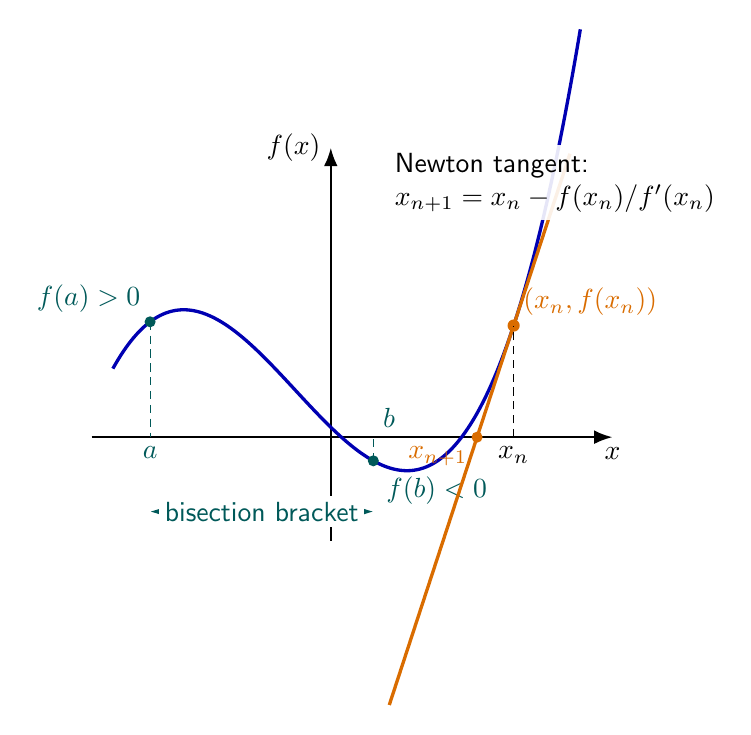
\begin{tikzpicture}[>=Latex,x=1.35cm,y=1.05cm,font=\sffamily]
  \draw[->,thick] (-2.25,0)--(2.65,0) node[below] {$x$};
  \draw[->,thick] (0,-1.25)--(0,3.5) node[left] {$f(x)$};
  \draw[very thick,blue!70!black,domain=-2.05:2.35,samples=180]
    plot (\x,{0.42*(\x)^3+0.42*(\x)^2-1.25*(\x)+0.12});
  \coordinate (A) at (-1.7,{0.42*(-1.7)^3+0.42*(-1.7)^2-1.25*(-1.7)+0.12});
  \coordinate (B) at (0.4,{0.42*(0.4)^3+0.42*(0.4)^2-1.25*(0.4)+0.12});
  \fill[teal!70!black] (A) circle (2pt) node[above left] {$f(a)>0$};
  \fill[teal!70!black] (B) circle (2pt);
  \draw[densely dashed,teal!70!black] (A)--(-1.7,0) node[below] {$a$};
  \draw[densely dashed,teal!70!black] (B)--(0.4,0) node[above right] {$b$};
  \node[teal!70!black,anchor=north west] at (0.43,-0.36) {$f(b)<0$};
  \draw[<->,teal!70!black,thick] (-1.7,-0.9)--(0.4,-0.9)
    node[midway,fill=white,inner sep=2pt] {bisection bracket};
  \pgfmathsetmacro{\xn}{1.72}
  \pgfmathsetmacro{\yn}{0.42*(\xn)^3+0.42*(\xn)^2-1.25*(\xn)+0.12}
  \pgfmathsetmacro{\slope}{1.26*(\xn)^2+0.84*(\xn)-1.25}
  \pgfmathsetmacro{\xnew}{\xn-\yn/\slope}
  \fill[orange!85!black] (\xn,\yn) circle (2.2pt) node[above right] {$(x_n,f(x_n))$};
  \draw[orange!85!black,very thick,domain=0.55:2.25]
    plot (\x,{\yn+\slope*(\x-\xn)});
  \draw[densely dashed] (\xn,0) node[below] {$x_n$}--(\xn,\yn);
  \fill[orange!85!black] (\xnew,0) circle (2pt) node[below left] {$x_{n+1}$};
  \node[align=left,anchor=west,fill=white,fill opacity=.9,text opacity=1,inner sep=3pt] at (0.52,3.08)
    {Newton tangent:\\$x_{n+1}=x_n-f(x_n)/f'(x_n)$};
\end{tikzpicture}
\end{document}
